\documentclass[14pt]{amsart}
%\usepackage{amsmath}
\usepackage[utf8]{inputenc}
\usepackage{graphicx}
\usepackage{xcolor}
\usepackage[legalpaper, margin=1.0in]{geometry}
\usepackage{fancyvrb}
\usepackage{cprotect}
\usepackage{url}
\usepackage{etoolbox}
\usepackage{hyperref}
\usepackage[skins,theorems]{tcolorbox}
\usepackage{enumitem}
\newcommand*{\vertbar}{\rule[-1ex]{0.5pt}{2.5ex}}
\newcommand*{\horzbar}{\rule[.5ex]{2.5ex}{0.5pt}}
\setlist[itemize]{align=parleft,left=1pt..1em}

\usepackage{imakeidx}
\makeindex


\usepackage{cmbright}
\usepackage[OT1]{fontenc}


% fonts
%\input{ArtNouvc.fd}
%\newcommand*\initfamily{\usefont{U}{ArtNouvc}{xl}{n}}
%\usepackage[T1]{fontenc}
%\usepackage{tgbonum} % change font

%\usepackage[light,condensed,math]{iwona}
%\usepackage[T1]{fontenc}

% from https://www.pinterest.co.uk/pin/88664686405122253/
\definecolor{C1}{RGB}{141, 125, 158} %purple
\definecolor{C2}{RGB}{163,156,147} % yellow
\definecolor{C3}{RGB}{99,151,153} % green
\definecolor{C4}{RGB}{195,106,99} % red
\definecolor{C5}{RGB}{124, 132, 128}
\definecolor{C6}{RGB}{67, 69, 75}


\definecolor{Gr}{HTML}{377D71}
\definecolor{Pu}{HTML}{A459D1}
\definecolor{Bl}{HTML}{4D455D}
\definecolor{Te}{HTML}{C1ECE4}
\definecolor{Or}{HTML}{EF6262}
\definecolor{Am}{HTML}{F3AA60}
\definecolor{Co}{HTML}{3C486B}
\definecolor{Wh}{HTML}{FEFBF6}
\definecolor{Ye}{HTML}{FFE196}
\definecolor{Re}{HTML}{E96479}
\definecolor{Pi}{HTML}{FFD0D0}
\definecolor{Rp}{HTML}{FF9EAA}
\definecolor{Wg}{HTML}{EEF3D2}


\hypersetup{
    colorlinks=false,
    linkcolor=red,
    filecolor=red,      
    urlcolor=red,
    pdftitle={a},
    pdfpagemode=FullScreen,
    }
    
    
 % TCOLORBOX STUFF ----------------------------------------------------------------------------
 

 %  ----------------------------------------------------------------------------
    
\patchcmd{\section}{\normalfont}{\color{C5}}{}{}
\patchcmd{\subsection}{\normalfont}{\color{C5}}{}{}


\newcommand{\dfn}[1]{{\bf  \color{blue}{#1}}}


\renewcommand{\FancyVerbFormatLine}[1]{\color{gray}{>\,\,#1}}
    
\newtheorem{thm}{Theorem}


\newtheoremstyle{exercise}
{}                % Space above
{}                % Space below
{\color{black}}        % Theorem body font % (default is "\upshape")
{}                % Indent amount
{\bfseries}       % Theorem head font % (default is \mdseries)
{:}               % Punctuation after theorem head % default: no punctuation
{ }               % Space after theorem head
{}                % Theorem head spec
\theoremstyle{exercise}
\newtheorem{exercise}{Exercise}


\newtheoremstyle{example}
{}                % Space above
{}                % Space below
{\color{red}\slshape}        % Theorem body font % (default is "\upshape")
{}                % Indent amount
{\bfseries}       % Theorem head font % (default is \mdseries)
{.}               % Punctuation after theorem head % default: no punctuation
{ }               % Space after theorem head
{}                % Theorem head spec
\theoremstyle{example}
\newtheorem{example}{Example}

\newtheoremstyle{solution}
{}                % Space above
{}                % Space below
{\color{C5}}        % Theorem body font % (default is "\upshape")
{}                % Indent amount
{\bfseries }       % Theorem head font % (default is \mdseries)
{:}               % Punctuation after theorem head % default: no punctuation
{\newline}               % Space after theorem head
{}                % Theorem head spec
\theoremstyle{solution}
\newtheorem*{solution}{Solution}


\newcommand{\mcS}{\mathcal S}
\newcommand{\mcR}{\mathcal R}
\newcommand{\mcC}{\mathcal C}
\newcommand{\bS}{{\boldsymbol S}}
\newcommand{\bR}{{\boldsymbol R}}
\newcommand{\bC}{{\boldsymbol C}}
\newcommand{\ba}{{\boldsymbol a}}
\newcommand{\bb}{{\boldsymbol b}}
\newcommand{\bs}{{\boldsymbol s}}
\newcommand{\bff}{{\boldsymbol f}}
\newcommand{\br}{{\boldsymbol r}}
\newcommand{\bx}{{\boldsymbol x}}
\newcommand{\bt}{{\boldsymbol t}}
\newcommand{\bv}{{\boldsymbol v}}
\newcommand{\bu}{{\boldsymbol u}}
\newcommand{\bw}{{\boldsymbol w}}
\newcommand{\bc}{{\boldsymbol c}}
\newcommand{\be}{{\boldsymbol e}}
\newcommand{\bq}{{\boldsymbol q}}
\newcommand{\bphi}{{\boldsymbol \phi}}
\newcommand{\brho}{{\boldsymbol \rho}}
\newcommand{\btau}{{\boldsymbol \tau}}
\newcommand{\reals}{\mathbb R}
\newcommand{\ints}{\mathbb N}
\newcommand{\E}{\mathbb E}
\newcommand{\Prob}{\mathbb P}


%%%%%%%%%%%%%%%




\begin{document}

\title{LLN, CLT, Normal models and linear regression}

\maketitle
\tableofcontents

\section{Reading}
\begin{itemize}
%\item Read section 2.4 from \cite{islp}.
\item Read chapter 4 of \cite{tabak}
\end{itemize}

\section{Learning objectives}

\begin{itemize}
\item The Central limit theorem (what it does and \underline{does not} tell us).
\item Working with Normal random variables (linear transformations of them, calculating probabilities). 
\item Correlation Normal random variables (Multivariate normal distribution). 
\item Basic linear regression model with a single predictor. 
\end{itemize}

\newif\ifhideproofs
%\hideproofstrue %uncomment to hide proofs

\ifhideproofs
\usepackage{environ}
\NewEnviron{hide}{}
\let\proof\hide
\let\endproof\endhide
\fi


  
  \section{The central limit theorem and sample distribution}
  
  
\begin{itemize}
\item We now have the formalism in place to state the Central Limit Theorem (CLT) in more precise terms. 
 \begin{thm} Let $X_i$ be a sequence of iid random variables and let 
 \begin{equation*}
E[X_i] = \mu,\quad  {\rm var}(X_i) = \sigma^2
 \end{equation*}
  and set 
  \begin{equation*}
 S_N = \sum_{i=1}^N X_i.
 \end{equation*}
 Then 
 \begin{equation}\label{eq:clt}
P\left( \frac{S_N-N\mu}{\sqrt{N \sigma^2}}<z\right) \to P(Z<z) 
 \end{equation}
Where
\begin{equation*}
Z \sim {\rm Normal}(0,1)
\end{equation*}
 \end{thm}
 \item The normal variable $Z$ with zero mean and variance one is called a \dfn{standard normal} random variable. Since evaluations of the CDF of a standard normal random variable appear so often, we use the shorthand 
 \begin{equation*}
 \Phi(z) = P(Z<z).
 \end{equation*}

 
\begin{example}[Binomial] Let 
\begin{equation*}
Y \sim {\rm Binomial}(N,q)
\end{equation*}


 \noindent
\underline{Question:} Assume $N$ is even and use the central limit theorem to approximate $P(Y<N/2)$ with a Normal distribution. How does the accuracy depend on $N$ and $q$? \\

 \noindent
\underline{Solution:} Using that $\mu = E[X_i] = q$ and $\sigma^2 = {\rm var}(X_i) = q(1-q)$, we find that the normal approximation to $Y$ is 
\begin{equation*}
P\left( \frac{Y - Nq}{\sqrt{N \sigma^2}} <z\right) \to P(Z<z)
\end{equation*}
for 
\begin{equation*}
Z \sim {\rm Normal}(0,1). 
\end{equation*}

Now we write
\begin{align*}
P\left( Y<N/2\right) &= P\left(Y - Nq <N/2-Nq\right) \\
&= P\left(\frac{Y - Nq}{\sqrt{N q(1-q)}} <\frac{N/2-Nq}{\sqrt{N q(1-q)}}\right)\\
&= P\left(\frac{Y - Nq}{\sqrt{N q(1-q)}} < \sqrt{N} \frac{1-2q}{2\sqrt{q(1-q)}}\right)\\
&\to P\left(Z < \sqrt{N} \frac{1-2q}{2\sqrt{q(1-q)}}\right) = \Phi\left( \sqrt{N} \frac{1-2q}{2\sqrt{q(1-q)}}\right)
\end{align*}


We can use \href{https://colab.research.google.com/drive/1_4zOruAWfJ3HQoIf9sjefk3z0APko94-?usp=sharing}{colab} to plot both sides of this equation. 
%Note that if $q=1/2$, 
%\begin{equation*}
% P\left(Z < \sqrt{N} \frac{1-2q}{2\sqrt{q(1-q)}}\right)
% = P(Z<0) = \frac{1}{2}
%\end{equation*}
%However, since only $N/2-1$ of the outcomes are strictly less than $1/2$, we have
%\begin{equation*}
%P(Y<N/2) = \frac{N/2-1}{N} = \frac{1}{2}-\frac{1}{N}
%\end{equation*}
%We could in principle correct for this -- it's called a continuity correction, but it only matter when $N$ is small. 
%
%
% 

%\item If we rearrange this equation 
%\begin{equation*}
%Y ``\approx" U =  \sqrt{N \sigma^2}Z + Nq
%\end{equation*}
%What is the distribution of $U$? 
%\begin{equation}
%P(U
%\end{equation}




\end{example}

%\item {\bf Accuracy of CLT approximation and relative vs. absolute error:} In order to better understand how the accuracy of the CLT approximation depends on $N$, we make some plots of the error between the probabilities estimated using the CLT and the true probabilities (which we know from the formula for the Binomial distribution). There are two ways we can measure error. First, we could just look at the difference between the two probabilities:
%\begin{equation*}
%\text{Absolute Error} = \left|P\left( Y>N/2\right) - P\left(Z < \sqrt{N} \frac{1-2q}{2\sqrt{q(1-q)}}\right)\right|
%\end{equation*}
%However, in many cases, what really care about is the error relative to the true probability. For example, if the probabilities are both very very small (say we are trying to estimate the chance we get $99$ our of $100$ heads), then it more important that the error is very small. Thus, we introduce the relative error
%\begin{equation*}
%\text{Relative Error} = \frac{\left|P\left( Y>N/2\right) - P\left(Z < \sqrt{N} \frac{1-2q}{2\sqrt{q(1-q)}}\right)\right|}{P\left( Y>N/2\right)}
%\end{equation*}
%
%
%\begin{figure}[h]
%\centering
%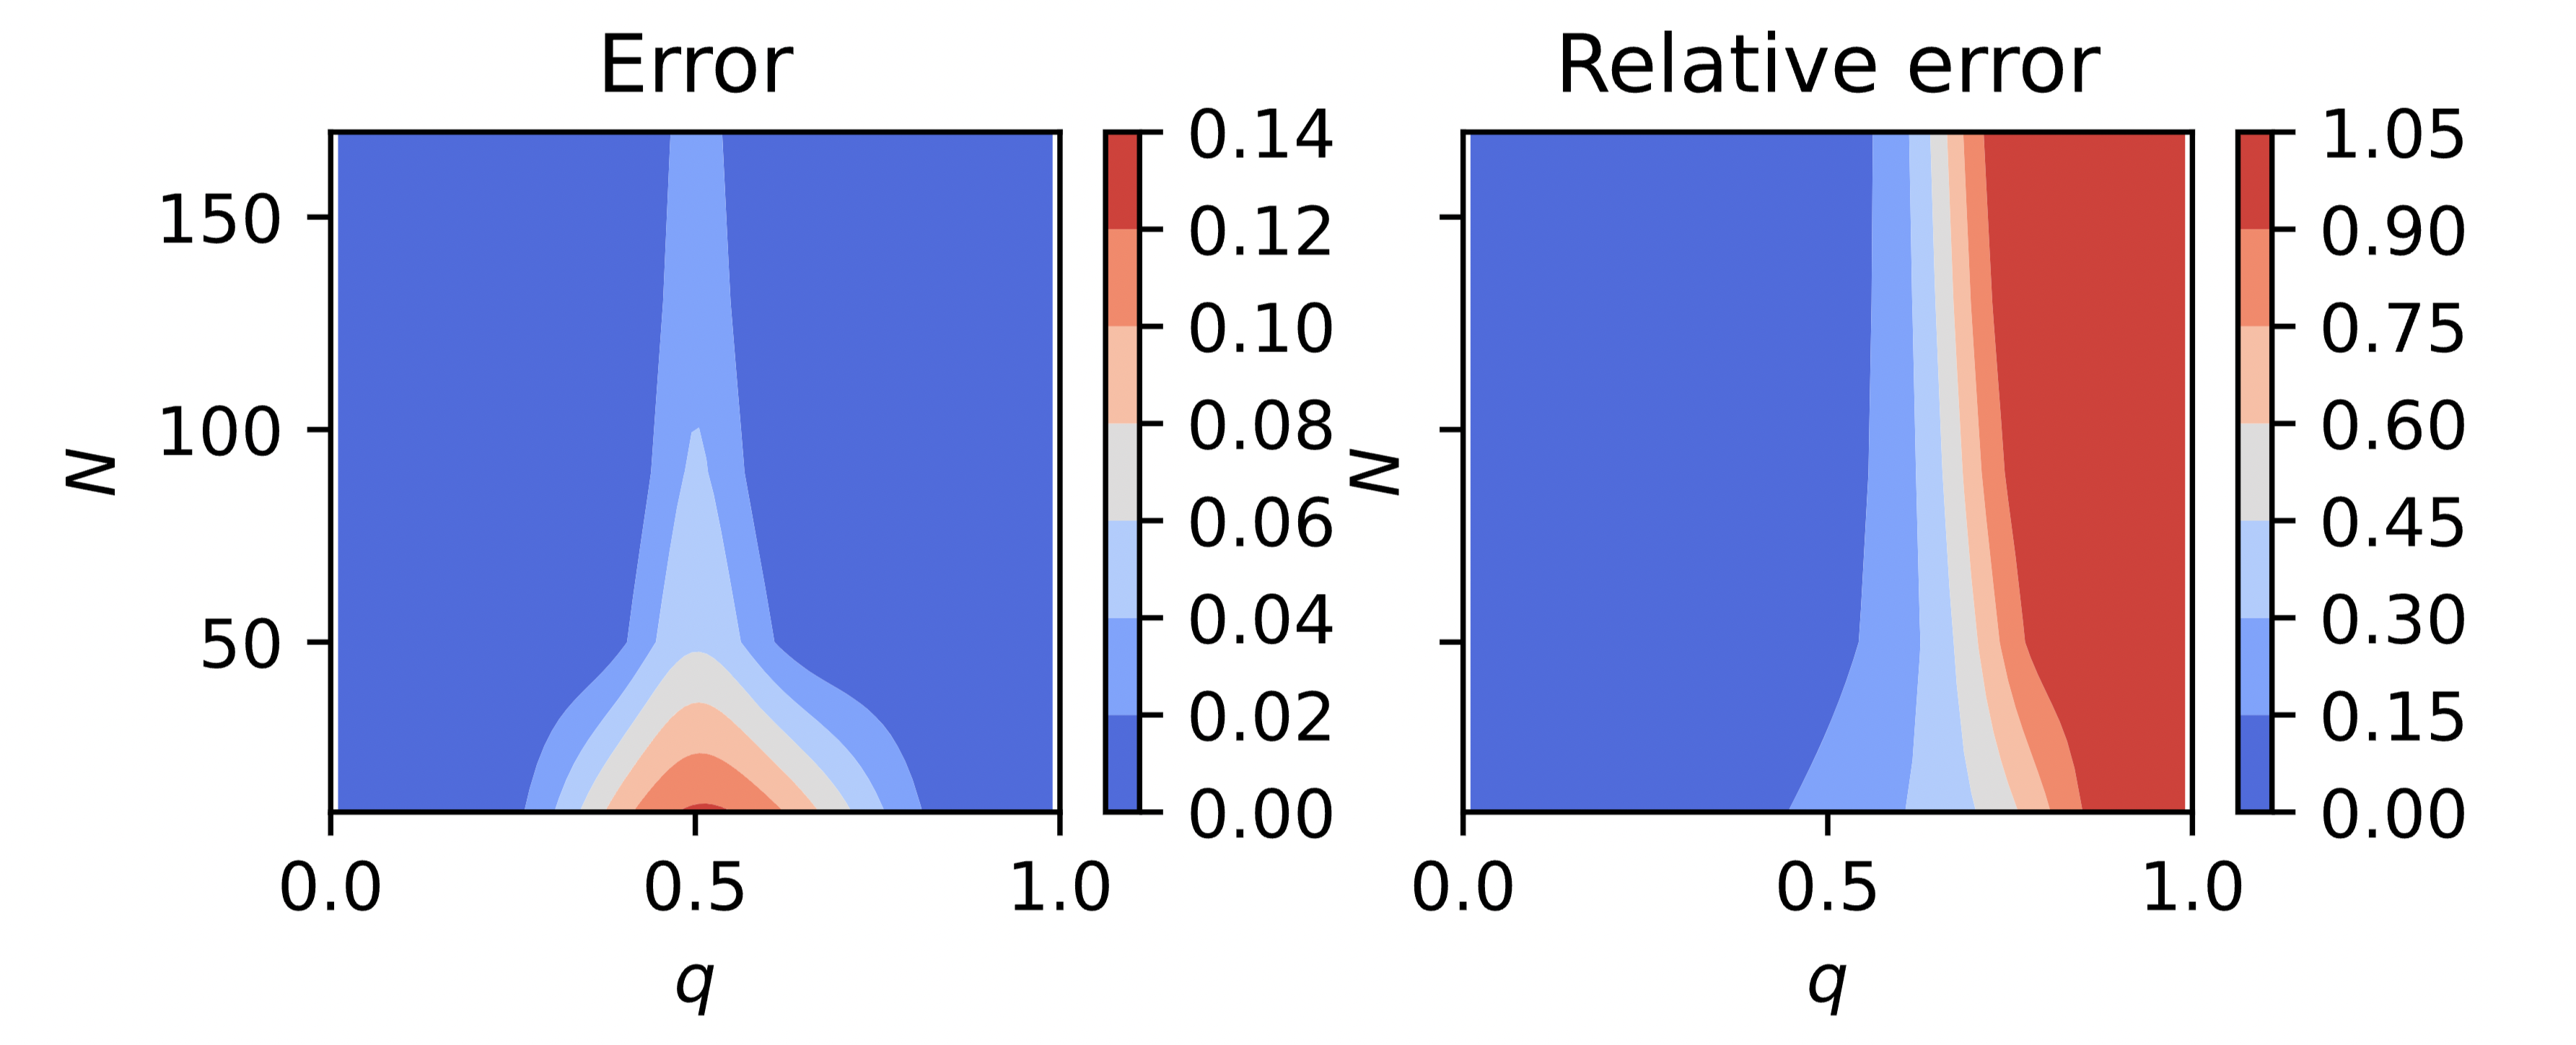
\includegraphics[width=0.6\textwidth]{./../figures/clt_binomial_err}
%\caption{The absolute (left) and relative error (right) are indicted by the color (red $=$ more error) as a function of $q$ and $N$.  }
%\end{figure}
%%




 %\item It is useful to define a more general class of Normal random variables with arbitrary mean and variance. Let's suppose we define a new variable 
%\begin{equation*}
%Y = \sigma Z + \mu 
%\end{equation*}
%Then 
%\begin{align*}
%P(Z<z) &= P(\mu + \sigma Z_0<z) \\
%&= P\left(Z<\frac{z - \mu}{\sigma}\right)\\
%&= \int_0^{\frac{z - \mu}{\sigma}}f_0(y)dy
%\end{align*}
%Setting $u = \sigma y + \mu$ so that $dy = \sigma^{-1}du$ we get
%\begin{equation*}
%P(Z<z) = \frac{1}{\sigma} \int_0^zf_0\left(\frac{u -\mu}{\sigma} \right)du = \int_0^zf(u)du 
%\end{equation*}
%where
%\begin{equation*}
%f(y) = \frac{1}{\sqrt{2\pi \sigma^2}}e^{-\frac{(y-\mu)^2}{2\sigma^2}}. 
%\end{equation*}
%We also call the random variable $Z$ and write
%\begin{equation*}
%Z \sim {\rm Normal}(\mu,\sigma^2).



\vspace{1cm}
\begin{center}
\textcolor{black}{{\bf \Huge Do Exercise 3}}
\end{center}
\vspace{1cm}

\item {\bf Note on iid assumption:} One of the most important things to recognize about the CLT when it comes to application is that the assumptions that the $X_i$ are independent are not that important, so long as they are not too correlated. Even though the precise quantitive statement of the CLT won't when there are correlations, the sum will still be well approximated by a Normal distribution. We can state this in what I call the qualitative CLT. This is a point we will return to later! 

\end{itemize} 


%
%
%
%\subsection{Central Limit Theorem}
%\begin{itemize}
%\item The \dfn{central limit theorem} tell us that when $y_i$ are independent and have a (finite) mean and variance $\mu_y$ and $\sigma_y$ and
%\begin{equation*}
% \hat{Y} = \frac{1}{N}\sum_{i=1}^Ny_i,
%\end{equation*}
%then the distribution of $\hat{Y}$ should be close to that of
%\begin{equation*}
%Y \sim {\rm Normal}(\mu_y,\sigma_y/\sqrt{N}).
%\end{equation*}
%\end{itemize}













\subsection{Properties of Normal random variables}
\begin{itemize}

\item {\bf Linear transformations of Normal random variables:}  Suppose 
\begin{equation*}
Z \sim {\rm Normal}(0,1)
\end{equation*}
and define 
\begin{equation*}
X = \sigma Z + \mu 
\end{equation*}
Then 
\begin{align*}
P(X<x) &= P(\mu + \sigma Z<x) \\
&= P\left(Z<\frac{x - \mu}{\sigma}\right)
%&= \int_0^{\frac{x - \mu}{\sigma}}f(x)dx
\end{align*}
%Setting $u = \sigma x+ \mu$ so that $dx = \sigma^{-1}du$ we get
%\begin{equation*}
%P(X<x) = \frac{1}{\sigma} \int_0^xf_0\left(\frac{x -\mu}{\sigma} \right)du = \int_0^xf(x)dx 
%\end{equation*}
%where
%\begin{equation*}
%f(x) = \frac{1}{\sqrt{2\pi \sigma^2}}e^{-\frac{(x-\mu)^2}{2\sigma^2}}. 
%\end{equation*}
Hence 
\begin{equation*}
X \sim {\rm Normal}(\mu,\sigma^2).
\end{equation*} 
\item With this understanding of how to linearly transform a Normal random variable, we can see that the CLT can be informally stated as
\begin{equation*}
S_N \approx S_{\rm CLT} \sim {\rm Normal}(N\mu,N\sigma^2)
\end{equation*}
\item More generally, 
\begin{equation*}
X \sim {\rm Normal}(\mu_x,\sigma_x)
\end{equation*}
Now consider 
\begin{equation*}\label{eq:linear}
Y = aX + b 
\end{equation*}
At this point it should make sense that $Y$ is also normal. 
 but what are the mean and variance? Taking the average of both sides, 
\begin{equation*}
E[Y] = a\mu + b
\end{equation*}
and 
\begin{equation*}
{\rm var}(Y) = {\rm var}(aX) + {\rm var}(b)
\end{equation*}
Form the formula for variance, we know ${\rm var}(aX)  = a^2{\rm var}(X)$. Also, ${\rm var}(b) =0$
So 
\begin{equation*}\label{eq:normal_linear_trans}
Y \sim {\rm Normal}(a\mu_x + b,a^2\sigma_x^2).
\end{equation*}
Note that in going from $Z$ to $X$ and $X$ to $Y$, we are just multiplying and shifting everything.
Think about what this does to the histogram. 
\item The process of going from $X$ to $Z$ is called standardizing. For any variable $X$ the \dfn{standardized} variable is defined as 
\begin{equation*}
Z = \frac{X-\mu_x}{\sigma_x}
\end{equation*}
 {\bf Transforming $X$ to a standard Normal is equivalent to measuring $X$ in units of standard deviations.} For example, if we make a histogram of $X$, all this transformation does is change the $X$ axis to units of standard deviations from the mean. 
 
%\item Another way to think about what the CLT theorem is saying is that 
%\begin{equation*}
% S_N \approx Z \sim {\rm Normal}(NE[X_i],N{\rm var}(X_i)).
%\end{equation*}
%That is, a sum over a large number of terms is ``approximately'' Normal with mean $NE[X_i]$ and variance $N{\rm var}(X_i)$. We will often refer to the this as the CLT approximation of a random variable. 


 \item {\bf Combing normal random variables:} Suppose
 \begin{align*}
Y_1 &\sim {\rm Normal}(\mu_1,\sigma_1^2)\\
Y_2 &\sim {\rm Normal}(\mu_2,\sigma_2^2)\\
\end{align*}
What is the distribution of $X_1+X_2$? One way to see that this should be Normal is to note that Normal random variables emerge form the CLT as sums over many (roughy) iid variables. Let's say $Y_1$ and $Y_2$ are respectively approximations to sums $S_1$ and $S_2$ over $N_1$ and $N_2$ terms. Let $f_X$ be the distribution of terms in the first sum and $f_{X'}$ the second. Then, if we sample a random term from the $N_1+N_2$ terms that make up the sum $S_1+S_2$, the chance that is was a sample from $f_{X}$ is $N_1/(N_1+N_2)$. The chance it come from $f_{X'}$ is $N_2/(N_1+N_2)$. Therefore, it has a distribution which is 
\begin{equation*}
f_X\frac{N_1}{N_1+N_2} + f_{X'}\frac{N_2}{N_1+N_2}.
\end{equation*}
If we draw another sample from these $N_1+N_2$ terms, its distribution will depend on the value of the first sample we obtained. For example, if samples from $f_X$ are very likely to take on very large values and $f_{X'}$, then a large value of the first sample we drew will tell us there are probably now less of the terms from the first sum in our list of $N_1+N_2$ numbers. However, the distribution of $S_1+S_2$ will still be approximately normal, since as we already mentioned, these correlations are not that important.  This is illustrated in Figure \ref{fig:clt_notiid}. 


\begin{figure}[h]
\centering
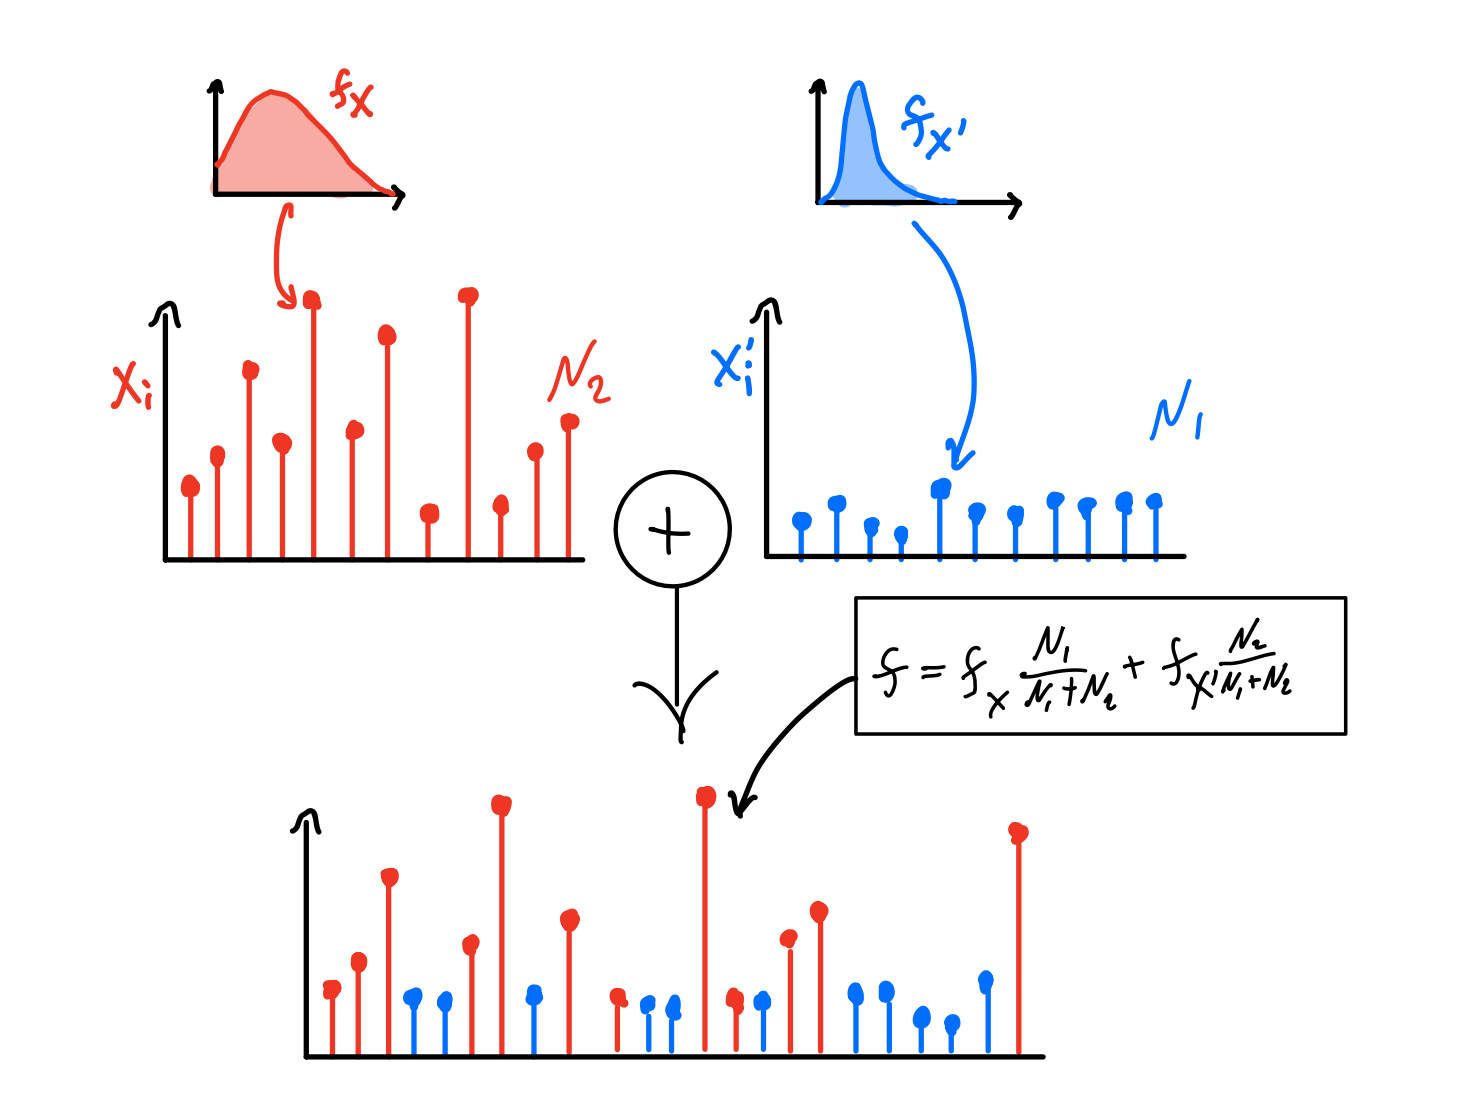
\includegraphics[width=0.8\textwidth]{./../figures/clt_notiid}
\caption{If we add two sums containing $N_1$ and $N_2$ terms respectively then the resulting sum behaves similar to the sum over $N_1 + N_2$ variables whose distribution is a mixture of the two. In particular, if we pick a random term from the sum, there is $N_1/(N_1+N_2)$ chance for it to follow the distribution of the first $N_1$ terms (denoted $f_X$ in the figure) and an $N_2/(N_1+N_2)$ chance for it to follow the second distribution.  }\label{fig:clt_notiid}
\end{figure}



 \item  We can summarize everything we learned above in the following result. 
 \begin{thm}[Special case of Theorem 4.6.1 in \cite{tabak}]\label{thm:addingnormal}
Let
\begin{align*}
X_1 &\sim {\rm Normal}(\mu_1,\sigma_1^2)\\
X_2 &\sim {\rm Normal}(\mu_2,\sigma_2^2)
\end{align*}
be independent, then 
\begin{equation*}
aX_1+bX_2 + d \sim {\rm Normal}\left(a\mu_1+b\mu_2+d,a^2\sigma_1^2 + b^2\sigma_2^2\right)
\end{equation*}
 \end{thm}
\end{itemize}


\section{Regression modeling}


\begin{itemize}
\item Now we want to understand relationships between Normal random variables. 
 \begin{example}[A taste of linear regression]\label{ex:firstreg}
Consider the following model:
\begin{align*}
X &\sim {\rm Normal}(\mu_x,\sigma_x^2)\\
Y|X &\sim {\rm Normal}(\beta_1X + \beta_0,\sigma^2)
\end{align*}

 \noindent
\underline{Question:} What is the marginal distribution of $Y$? What is $E[XY]$? How does this compare to $E[X]E[Y]$?\\


 \noindent
\underline{Solution:} We know that 
\begin{equation*}
Y|X =\beta_1X+\beta_0 + Z,\quad Z \sim {\rm Normal}(0,\sigma^2)
\end{equation*}
Thus, the marginal distribution of $Y$ is the sum of two Normal random variables with mean and variance $(\beta_1\mu_x+\beta_0,a\sigma_x^2)$ and $(0,\sigma^2)$ respectively. 
By Theorem \ref{thm:addingnormal}, 
\begin{equation*}
Y  \sim {\rm Normal}(\beta_1\mu_x+\beta_0,\beta_1^2\sigma_x^2 + \sigma^2)
\end{equation*}

To compute $E[XY]$, we note that 
\begin{equation*}
E[XY|X=x]=  E[xY|X=x]= xE[Y|X=x]
\end{equation*}
therefore
\begin{equation*}
E[XY] = E[XE[Y|X]] = E[X(\beta_1X+\beta_0)] = \beta_1E[X^2]+\beta_0E[X]
\end{equation*}
Using 
\begin{equation*}
E[X^2] = {\rm var}(X) + E[X]^2 = \sigma_x^2 + \mu_x^2
\end{equation*}
Therefore 
\begin{equation*}
E[XY] =  \beta_1\sigma_x^2 + \beta_1\mu_x^2 + \beta_0\mu_x
\end{equation*}
On the other hand, 
\begin{equation*}
E[X]E[Y] = \mu_x(\beta_1\mu_x+\beta_0) = \beta_1 \mu_x^2 +\beta_0 \mu_x
\end{equation*}
The difference between the two is the additional term $\beta_1\sigma_x^2$, which we picked up from the variance of $x$.  


\end{example}

\item The example above motivates the definition of \dfn{covariance}
\begin{equation}
{\rm cov}(X,Y) = E[XY]-E[X]E[Y]
\end{equation}
Note that another way to write this is 
\begin{equation*}
 E[(Y-E[Y])(X-E[X)] = E[XY] - 2E[X]E[Y]+E[X]E[Y] = {\rm cov}(X,Y)
\end{equation*}
so if we replaced $X$ with $Y$, this becomes the variance. 
\item We can generalize the relationship between the covariance, slope $(a)$ and variance of $X$ $(\sigma_x^2)$ in Example \ref{ex:firstreg} to any model of the form 
\begin{align}
\begin{split}\label{eq:linreg}
X &\sim \text{some distribution with mean $\mu_x$ and variance $\sigma_x^2$}\\
Y|X &\sim {\rm Normal}(\beta_1X + \beta_0,\sigma^2). 
\end{split}
\end{align}
Such a model is a linear \dfn{linear regression model}. The variable $X$ is called the \dfn{predictor} and $Y$ the \dfn{response} variable. 
Recall that we can write $E[X^2]$ as
\begin{equation*}
E[X^2] ={\rm var}(X) + E[X]^2 =  \sigma_x^2 + \mu_x^2. 
\end{equation*}
Now for any linear regression model
\begin{align*}
E[XY] &= E[XE[Y|X]] = E[X(\beta_1 X+\beta_0)] = \beta_1E[X^2] + \beta_0 E[X] \\
&= \beta_1\sigma_x^2 +\beta_1 \mu_x^2 +\beta_0 \mu_x\\
E[Y] &= \beta_1\mu_x +\beta_0
\end{align*}
so 
\begin{align*}
{\rm cov}(X,Y) &= \beta_1\sigma_x^2
\end{align*}
regardless of the distribution of $X$ (assuming $\sigma_x^2 <\infty$). The intuition for this formula is given in figure \ref{fig:cov_effect}. 


\begin{figure}[h]
\centering
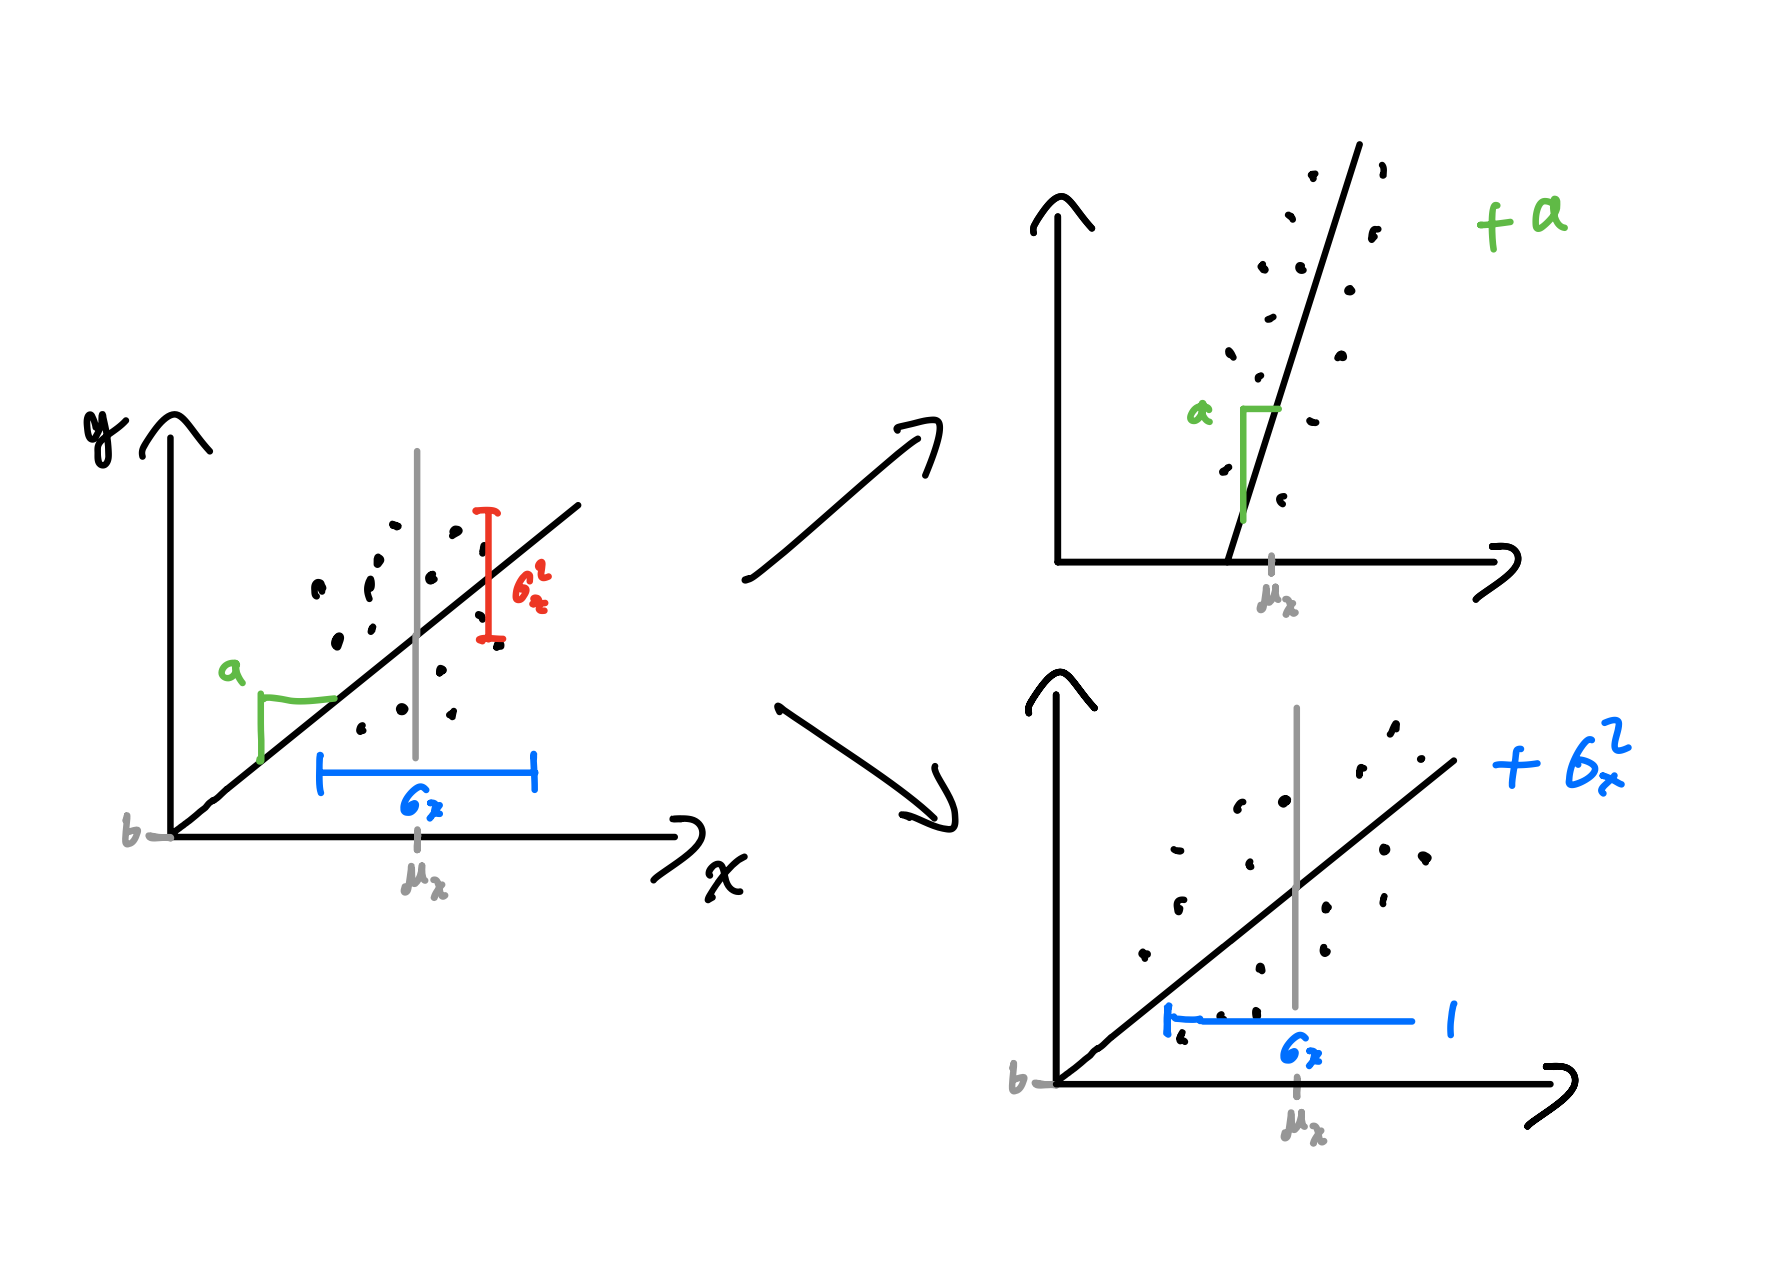
\includegraphics[width=0.8\textwidth]{./../figures/cov_effect}
\caption{}\label{fig:cov_effect}
\end{figure}




\vspace{1cm}
\begin{center}
\textcolor{black}{{\bf \Huge Do Exercises 4 an 5}}
\end{center}
\vspace{1cm}


\item A crucial observation is that the covariance allows us to relate the parameter $\beta_1$ (the slope) in the model above to averages over $X$ and $Y$. In other words, it provides us with a means to estimate the slope from samples $(x_1,y_2),\dots,(x_n,y_n)$. 
\begin{align*}
 \beta_1 &\approx  \frac{\sum_{i=1}^n\left(x_i - \bar{X}\right)\left(y_i-\bar{Y}\right)}{\sum_{i=1}^n\left(x_i - \bar{X}\right)^2}
\end{align*}
The is what the function 
\begin{Verbatim}
np.cov(x,y)[0,1]
\end{Verbatim}
computes in Python. 
The reason for the $[0,1]$ is that the covariance function in numpy actually computes a 2D array (a Matrix), where the off diagonal entries are the covariance. The diagonal entries are the variances. 

We can also estimate $\beta_0$. Using $E[Y] = \beta_1 \mu_x + \beta_0$ we have
\begin{equation*}
\beta_0 =  E[Y]  - \beta_1 \mu_x \approx \hat{\beta}_0 =  \overline{Y} - \left(\frac{\sum_{i=1}^n\left(x_i - \bar{X}\right)\left(y_i-\bar{Y}\right)}{\sum_{i=1}^n\left(x_i - \bar{X}\right)^2}\right)\overline{X}
\end{equation*}

%\item In exercise 5 you saw that even when both $X$ and $Y$ are normally distributed, we will get a different estimate of $\beta_1$ depending on 

\end{itemize}

\subsection{Least square interpretation}
\begin{itemize}
\item Suppose we plot $X$  and $Y$ points in a place. Regardless of where these $X$ and $Y$ points come from (Normal model or not), we can compute $\hat{\beta}_1$ and $\hat{\beta}_0$. 
These estimators are known as \dfn{least squares} estimators (note that we haven't formally defined what an estimator is) because  it happens that these values minimize the sum of the squared difference between our data points and the line $\hat{a}x + \hat{b}$. That is, they are the values that make the \dfn{residual sum of squares}(RSS) smallest
\begin{equation*}
RSS = \sum_{i=1}^n r_i^2,\quad r_i  = Y_i - (\hat{\beta}_1X_i + \hat{\beta}_0)
\end{equation*}
smallest. The R

\begin{figure}[h]
\centering
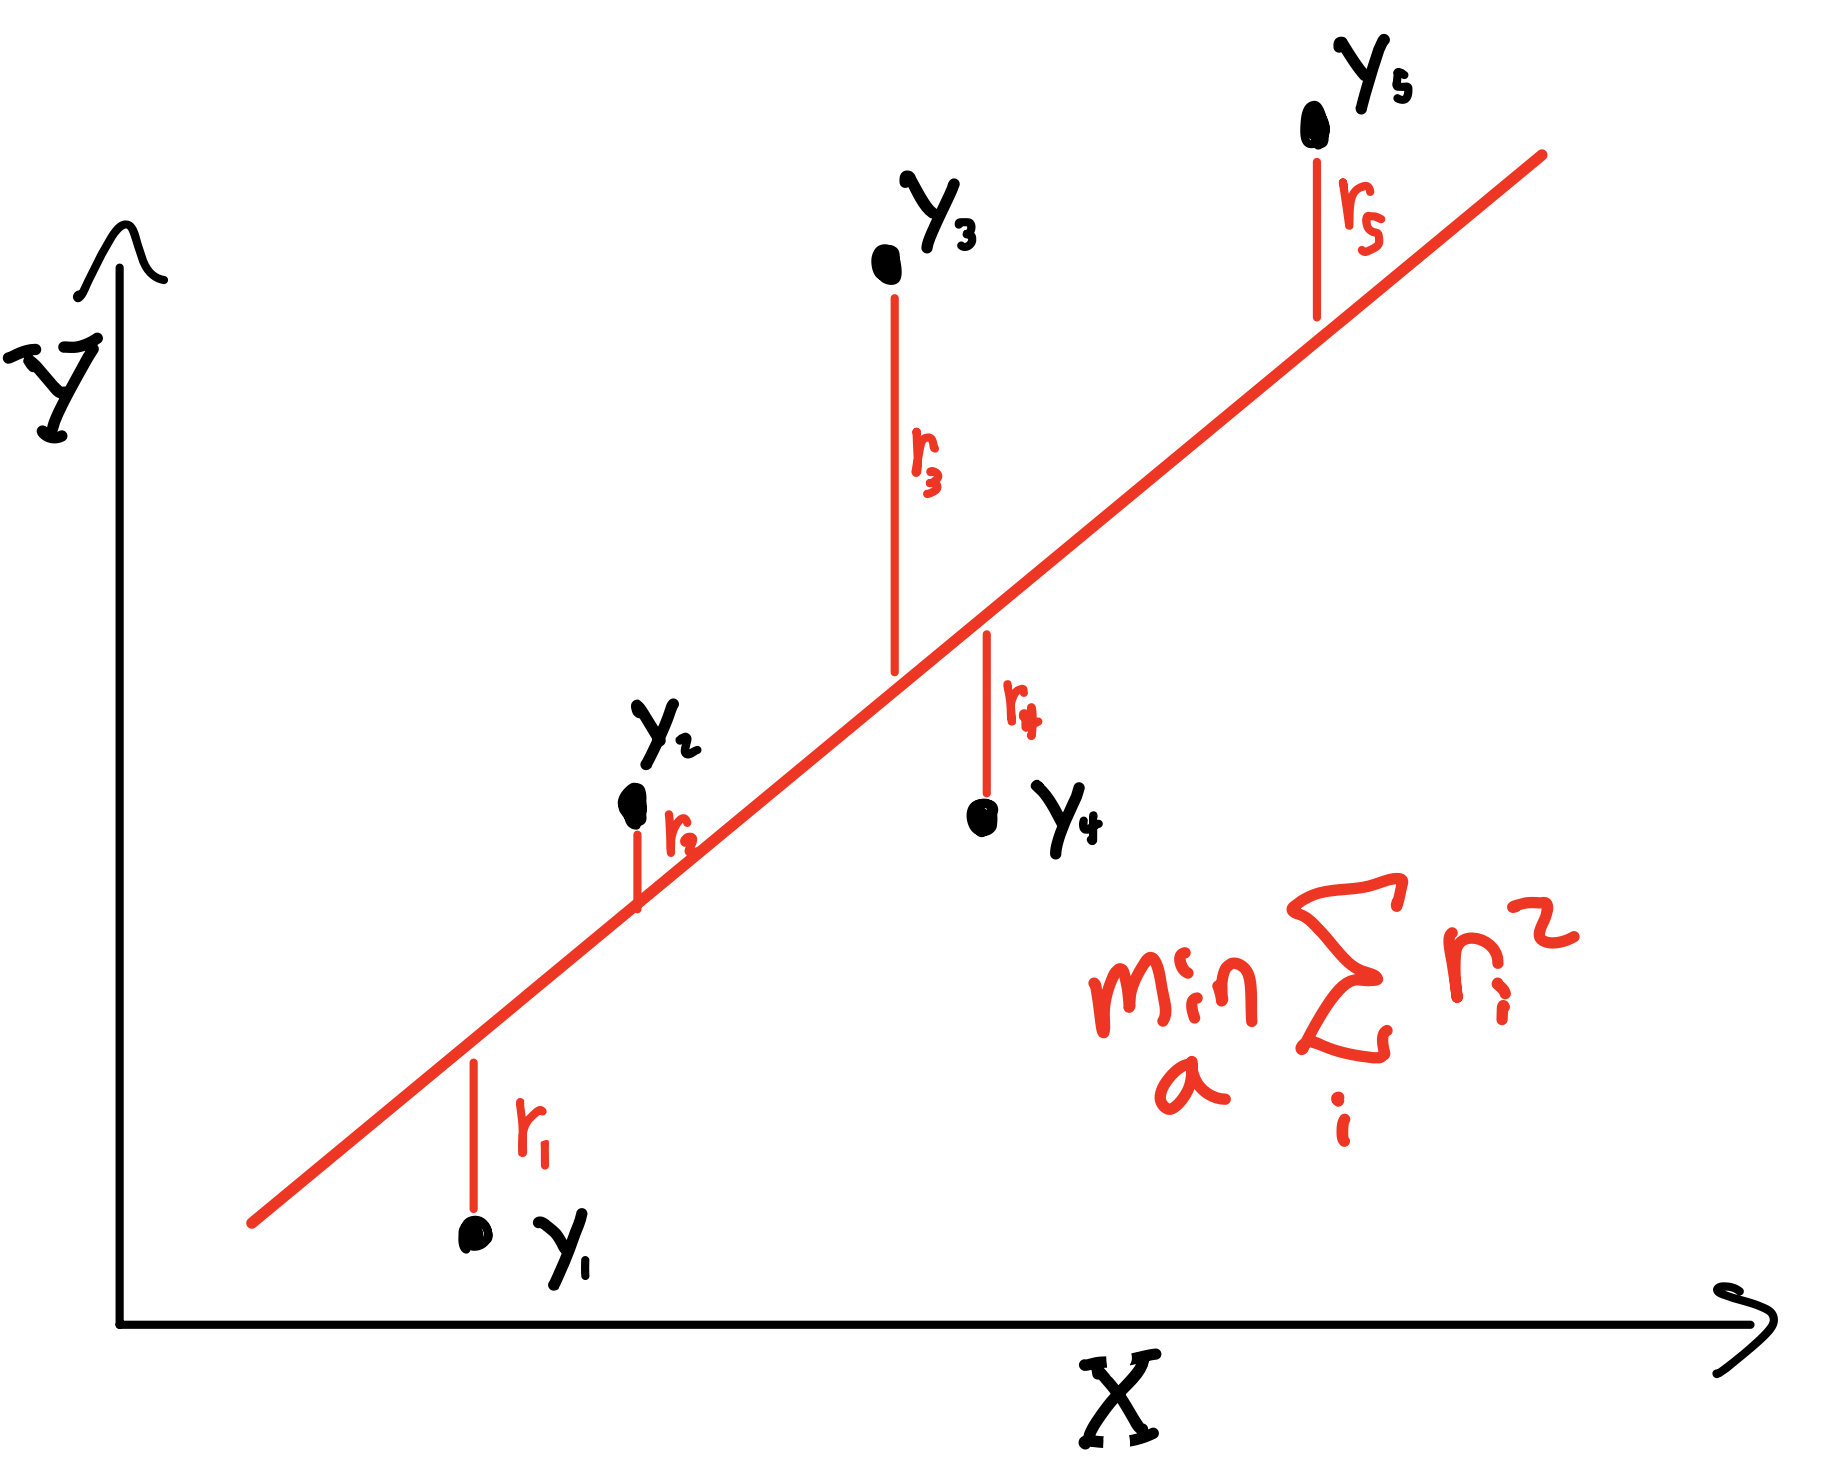
\includegraphics[width=0.4\textwidth]{./../figures/rss}
\caption{ }\label{rss}
\end{figure}


There are many other ways we could draw a line through a set of $(x,y)$ points. This particular way of estimating the slope -- by minimizing RSS -- happen to make sense under the assumption that  the data is sampled from a Linear regression model (Equation \ref{eq:linreg}). 

%\begin{example}[A taste of statistical inference] One the main applications of the CLT in this course is to access the accuracy of our estimates of parameters from iid samples. 
%\begin{equation*}
%T \sim {\rm Exponential}(\lambda)
%\end{equation*}
%We know that $E[T] = \tau = 1/\lambda$, so to estimate $\tau$ from samples $T_1,\dots,T_n$ we would do 
%\begin{equation*}
%\tau \approx \bar{\tau} = \frac{1}{n} \sum_{i=1}^nT_i
%\end{equation*}
%Since $\bar{\tau}$ depends on the data we collect, different replications of our sample will generate different values of $\bar{\tau}$. We call these replicates of the data and distribution of $\bar{\tau}$ taken over many replications of the data is our sample distribution. \\
%% We can therefore think of $\hat{\tau}$ as a random variable itself.  We call the distribution of $\hat{\tau}$ over many replications of our data the \dfn {sample distribution}. I will use \dfn{replicate} to mean different realizations of our data (as opposed to the different samples within the data). The sample distribution is the distribution of $\hat{\mu}$ over many replicates, but each replicate involves many samples. \\
%
%
% \noindent
%\underline{Question:} If $\tau=1$, then how many samples do we need to collect in order for the standard deviation in our estimate of $\bar{\tau}$ between experiments to be less that $0.1$ of the mean? \\
%
% \noindent
%\underline{Solution:} 
%By the CLT and the fact that ${\rm var}(T) = \tau^2$, 
%\begin{equation*}
%\bar{\tau} =\frac{1}{n} \sum_{i=1}^nT_i  
%\end{equation*}
%is approximately 
%\begin{equation*}
%{\rm Normal}\left(\tau, \frac{\tau}{\sqrt{n}} \right)
%\end{equation*}
%We want $\tau/\sqrt{n} = 1/\sqrt{n}<0.1 \implies 10^2  = 100 <n$. 
%
%\end{example}

 % ------------------------------------------------------------------------------------------------------------------------------------------
\begin{example}[Marketing data]
Here we consider the some on advertising budgets and sales for a company. We will explore whether the budget for TV advertisements is associated with higher sales. \\

 \noindent
\underline{Questions:} Fit the data to a linear regression model with the TV budget at the  predictor and sales as the response variable. 
\begin{enumerate}[label=(\alph*)]
\item {\bf Fit linear regression model:} What are the estimates of $\beta_1$ and $\beta_0$? 
\item {\bf Visualize the data:} Plot the regression long along with a scatter plot of the data. 
%\item {\bf A rudimentary hypothesis test:}  Suppose that in reality, $\beta_1=0$. This means $\beta_0 = \mu_y$ since 
%\begin{equation*}
%\mu_y = E[Y] = \beta_1 \mu_x + \beta_0 = \beta_0.
%\end{equation*}
%Estimate $\mu_y$ and simulate $10000$ ``fake'' data sets under the assumption that $\beta_0$. For each one, estimate the slope and save it in an array. Based on these estimates, what is the chance that we obtain a value of $\beta_1$ which is at least at large as the one we obtained from the real data? This will tell us if it is possible our estimated $\hat{\beta_1}$ is positive only by accident. 
\item {\bf Accessing model assumptions:} Using the fitted values of $\beta_1$ and $\beta_0$, simulate $10$ ``fake'' data sets which have the same number of points as the real data set and the same $x$ values.  Make plots of these and compare to the real data.  \\
\end{enumerate}

 \noindent
\underline{Solution:} see \href{https://colab.research.google.com/drive/1_4zOruAWfJ3HQoIf9sjefk3z0APko94-?usp=sharing}{colab} notebook. 
\end{example}



 % ------------------------------------------------------------------------------------------------------------------------------------------
%\begin{example}[Test scores -- regression with a binary predictor]
%Let's consider again the example of test score: We have data on test scores and mother high school education.  
%Aside from mother high school education,  variation in scores between students is presumably dependent on many roughly independent things, from other aspects of their home environment to their mood at the time of the test. It is therefore a natural to model the distribution of test scores (conditioned on mother high school education) as a Normal random variable. 
%We will use the regression model 
%\begin{equation*}
%Y|X \sim {\rm Normal}(\beta_1  X + \beta_0,\sigma_{\epsilon}^2)
%\end{equation*}
%where $\sigma_{\epsilon}^2 = \sigma_{Y|X}^2$. 
%This is usually written as
%\begin{equation*}
%Y= \beta_1 X + \beta_0 + \epsilon 
%\end{equation*}
%with the understanding that 
%\begin{equation*}
% \epsilon  \sim {\rm Normal}(0,\sigma_{\epsilon}^2). 
%\end{equation*}
%We could also write an equation for $X$: 
%\begin{equation*}
%X \sim {\rm Bernoulli}(q),
%\end{equation*}
%although we usually think of the equation for $Y|X$ as the regression model.   \\
%
% \noindent
%\underline{Question:}
%\begin{itemize}
%\item What are the estimates of $\beta_1$ and $\beta_0$? 
%\item How are these related the conditional averaged we have discussed earlier? 
%\item Generate simulated data based on this model. 
%\item Based on this regression model, what is our best prediction for the chance that a student whose mother attended high school got a score greater than $100$?\\
%\end{itemize}
%
%
% \noindent
%\underline{Solution:} see \href{https://colab.research.google.com/drive/1_4zOruAWfJ3HQoIf9sjefk3z0APko94-?usp=sharing}{colab} notebook. 
%\end{example}
%
%
%\end{itemize}

\end{itemize}





%\section{Linear regression model}
%\begin{itemize}
%\item Example \ref{} is a special case of a \dfn{regression model}. We now introduce the concept of regression modeling. 
% A very broad class of models in statistics for the relationship between two variables $X$ and $Y$ is a regression model:
%\begin{equation*}
%Y = f(X) + \epsilon
%\end{equation*}
%where $f$ is a deterministic function; that is, if we evaluate $f$ at a particular number, we get something that is not random. The term $\epsilon$ represents some source of noise {\bf independent of $X$}, and is typically modeled with a Normal distribution
%\begin{equation*}
%\epsilon \sim {\rm Normal}(0,\sigma_{\epsilon}).
%\end{equation*}
%In other words, it represents things other than $X$ which may influence $Y$.
%Regardless of how $X$ is distributed, for any given values $X=x$, $Y$ must have a Normal distribution:
%\begin{equation*}
%Y|(X=x) \sim {\rm Normal}(f(x),\sigma_{\epsilon}). 
%\end{equation*}
%
%\item Of particular interest (due to its simplicity) is the case
%\begin{equation}
%f(x) = ax + b
%\end{equation}
%which is the subject of this class. That is, we are interested in the model
%\begin{equation}\label{eq:lin_reg}
%Y =  aX + b + \epsilon
%\end{equation}
%where 
%\begin{equation}
%\epsilon \sim {\rm Normal}(0,\sigma_{\epsilon}). 
%\end{equation}
% $X$ and $Y$ are not independent. This can be seen visually.  {\bf Note: even though $X$ and $Y$ are not independent, we don't say they effect each other. To see why this terminology is problematic note that $Y$ has no ``effect" on $X$ (it is determined by $X$). However, what is $X|Y=y$?}
%\end{itemize}

%\subsection{Working with regression}
%
%\begin{itemize}
%\item In Equation \eqref{eq:lin_reg}, $X$ could be anything, but let's suppose $X$ is drawn from a Normal distribution. 
%This gives us the model 
%\begin{align}\label{eq:wwr}
%Y &=  aX + b + \epsilon\\
%X &\sim {\rm Normal}(\mu_x,\sigma_x)
%\end{align}
%(technically this is not a regression model anymore because we specify the distribution of $X$). 
%\item Now that we have two random variables, we can ask questions like, what is the joint distribution? what are the conditional distributions? What are the Marginal distributions? 
%Using properties of Normal random variables, we get 
%\begin{equation}
%Y \sim {\rm Normal}(a\mu + b,\sqrt{a^2\sigma_x^2 + \sigma_{\epsilon}^2})
%\end{equation}
%This is the distribution of $Y$ regardless of $X$; that is, it is the distribution we would get if we randomly sampled $Y$ values ignoring what the value of $X$ is. What is another name for this? 
%This distribution can be understood visually
%\item
% \end{itemize}
 
%Remember that when we condition on $X$ we get back the regression model. 
%\begin{equation}
%Y|(X=x) \sim {\rm Normal}(ax + b,\sigma_{\epsilon})
%\end{equation}
%\subsection{Autoregressive model}
%\begin{itemize}
%\item A common application of regression of regression models is to model time-series data. Suppose we have a sequence of Temperature observations 
%\begin{equation}
%X_1,X_2,X_3,\dots
%\end{equation}
%We want to model the randomness in $X_i$ while accounting for the fact that $X_{i-1}$ depends on the previous values in some way.
%An autoregressive model is one where this done by via a linear regression with $X_i$ as the response and $X_{i-1}$ as the predictor; that is
%\begin{equation*}
%X_i|X_{i-1} \sim {\rm Normal}(aX_{i-1}+b,\sigma^2)
%\end{equation*}
%\item If the marginal distribution of $X_i$ is the same for all $i$, then we say that the process is stationary. Under what conditions does this happen? 
%\end{itemize}


%\subsection{Least squares as solving linear equations}
%\begin{itemize}
%\item Another common way to think about least squares is as solving a linear system of equations. Let 
%\begin{equation}
%(X_1,Y_1),\dots,(X_N,Y_N)
%\end{equation}
%be our data. 
%We want to find a line that passes through this data and is, in some sense, close to the points. 
%\begin{align*}
%Y_1 &= aX_1 + b\\
%Y_2 &= aX_2 + b\\
%&\vdots\\
%Y_N &= aX_N + b\\
%\end{align*}
%In this equation there are two unknowns, $a$ and $b$, but $N$ equations. 
%We can write this matrix notation as 
%\begin{equation*}
%\left[ \begin{array}{c} Y_1\\ Y_2 \\ \vdots \\ Y_N\end{array}\right]
% =\left[ \begin{array}{cc}
% X_1 & 1\\
% X_2 & 1\\
% &\vdots \\
% X_N & 1
%  \end{array}\right]\left[ \begin{array}{c} a \\ b\end{array}\right]
%\end{equation*}
%
%\end{itemize}




%\subsection{Interpretation of regression parameters}
%The interpretation of parameters in regression model is important. Sometimes (the example below) there is a clear meaning in terms of conditional distributions, but suppose we have a model of our time in a race as a function of the temperature:  
%\begin{equation}
%Y = aX + b + \epsilon
%\end{equation}
%Let's start with $a$: This is the average difference between times for races at temperature which differ by $1$. (we expect this should be negative). $\epsilon$ is the variation around this average. Now what about $b$? The problem is that if we plug in $X=0$ we obtain a nonsensical quantity, so really $b$ does not have physical interpretation. This is common situation with regression models, and for this reason it is sometimes advantageous to center $X$. 






 \bibliographystyle{unsrt}
\bibliography{./../refs.bib}


\end{document}